% -*- coding: utf-8 -*-
% CSU Beamer: minimalist Central South University presentation template.
% Compile with XeLaTeX (or latexmk -xelatex main.tex).
\documentclass[10pt,aspectratio=169,hyperref={colorlinks,citecolor=csu_blue,urlcolor=csu_blue,linkcolor=}]{beamer}

\usepackage{CSU}
\usefonttheme{serif}
\usepackage{ctex}
\usepackage{hyperref}
\usepackage{lipsum}
\usepackage{latexsym,amsmath,xcolor,multicol,booktabs,calligra}
\usepackage{amssymb,graphicx,tikz,bm,natbib,wrapfig,amsfonts,ragged2e,parskip}

% 中文正文：优先使用 macOS 宋体，其他环境回退到 TeX Live 自带字体。
\IfFontExistsTF{Songti SC}{%
  \setCJKmainfont{Songti SC}[AutoFakeSlant=0.2]%
  \setCJKsansfont{Songti SC}[AutoFakeSlant=0.2]%
  \setCJKmonofont{Songti SC}%
}{%
  \setCJKmainfont{FandolSong-Regular}[Extension=.otf,BoldFont=FandolSong-Bold,AutoFakeSlant=0.2]%
  \setCJKsansfont{FandolSong-Regular}[Extension=.otf,BoldFont=FandolSong-Bold,AutoFakeSlant=0.2]%
  \setCJKmonofont{FandolFang-Regular}[Extension=.otf,BoldFont=FandolFang-Regular]%
}
\setmainfont{XCharter}
\IfFontExistsTF{Maple Mono NF}{%
  \setmonofont{Maple Mono NF}[Scale=MatchLowercase,Ligatures=TeX]%
}{%
  \IfFontExistsTF{Maple Mono}{\setmonofont{Maple Mono}[Scale=MatchLowercase,Ligatures=TeX]}{}%
}

\apptocmd{\frame}{}{\justifying}{}

% 让引用整体使用中南蓝（包括 natbib 生成的括号）。
\makeatletter
\NewCommandCopy{\csu@citep@orig}{\citep}
\NewCommandCopy{\csu@citet@orig}{\citet}
\RenewDocumentCommand{\citep}{o o m}{%
  \begingroup\color{csu_blue}%
  \IfNoValueTF{#1}{\csu@citep@orig{#3}}%
    {\IfNoValueTF{#2}{\csu@citep@orig[][#1]{#3}}{\csu@citep@orig[#1][#2]{#3}}}%
  \endgroup}
\RenewDocumentCommand{\citet}{o o m}{%
  \begingroup\color{csu_blue}%
  \IfNoValueTF{#1}{\csu@citet@orig{#3}}%
    {\IfNoValueTF{#2}{\csu@citet@orig[][#1]{#3}}{\csu@citet@orig[#1][#2]{#3}}}%
  \endgroup}
\makeatother

\newcommand{\theHalgorithm}{\arabic{algorithm}}
\theoremstyle{plain}
\newtheorem{axiom}{Axiom}
\newtheorem{claim}[axiom]{Claim}
\newtheorem{assumption}{Assumption}
\newtheorem{remark}{Remark}
\newtheorem{proposition}{Proposition}
\setbeamertemplate{theorems}[numbered]

\title[CSU Beamer]{CSU Beamer}
\subtitle{A minimalist Beamer template for Central South University}
\author[Central South University]{你的姓名\\{\small\href{mailto:your.name@csu.edu.cn}{\texttt{your.name@csu.edu.cn}}}}
\institute{中南大学 · 你的学院}
\date{\today}

\begin{document}

{\setbeamertemplate{logo}{}
\begin{frame}
  \titlepage
  \begin{figure}[htpb]
    \centering
    
\includegraphics[width=0.38\linewidth]{figures/logo.png}
  \end{figure}
\end{frame}}

\section{模板简介}

\begin{frame}{中文支持示例}
中南大学（Central South University）是一所以工学见长、学科门类齐全的综合性研究型大学。

\begin{itemize}
  \item 中文正文采用衬线宋体，英文采用 XCharter，适合学术汇报与答辩
  \item 每页底部保留作者、标题和页码信息，顶部导航与章节结构清晰
  \item 背景使用中南大学校徽淡色纹理，正文区域保持良好的可读性
  \item 数学公式：$\int_0^\infty e^{-x^2}\,\mathrm{d}x = \frac{\sqrt{\pi}}{2}$
\end{itemize}

\begin{theorem}[示例定理]
若函数 $f(x)$ 在闭区间 $[a,b]$ 上连续，则 $f(x)$ 在 $[a,b]$ 上必有最大值与最小值。
\end{theorem}
\end{frame}

\begin{frame}{研究背景与问题}
\begin{block}{统一的视觉语言}
模板采用轻量布局、固定高度顶栏、标题栏与三线表设计，并使用中南大学视觉元素。
\end{block}

\begin{itemize}
  \item 主题色：中南蓝（RGB 25, 98, 153）
  \item 校徽：使用 `figures/logo.png`，可直接替换为同尺寸资源
  \item 页面背景：使用 `figures/background.png`，每一页自动加载
\end{itemize}
\end{frame}

\section{内容示例}

\begin{frame}{数学表达式}
\begin{equation}
  \bm Y = \bm G\bm X + \bm E,
\end{equation}
其中 $\bm G\in\mathbb{R}^{N\times S}$ 为增益矩阵，$\bm E$ 为独立同分布的高斯误差。

\begin{align}
  \mathcal{L}(\theta) &= \frac{1}{n}\sum_{i=1}^{n}\ell(f_\theta(x_i),y_i),\\
  \theta^* &= \arg\min_\theta \mathcal{L}(\theta).
\end{align}
\end{frame}

\begin{frame}{表格与图片}
\begin{columns}[T]
  \column{.48\textwidth}
  \begin{table}
    \caption{示例数据}
    \centering
    \begin{tabular}{lrr}
      \toprule
      指标 & 方法 A & 方法 B \\
      \midrule
      准确率 & 0.91 & 0.94 \\
      召回率 & 0.88 & 0.92 \\
      \bottomrule
    \end{tabular}
  \end{table}
  \column{.48\textwidth}
  \begin{figure}
    \centering
    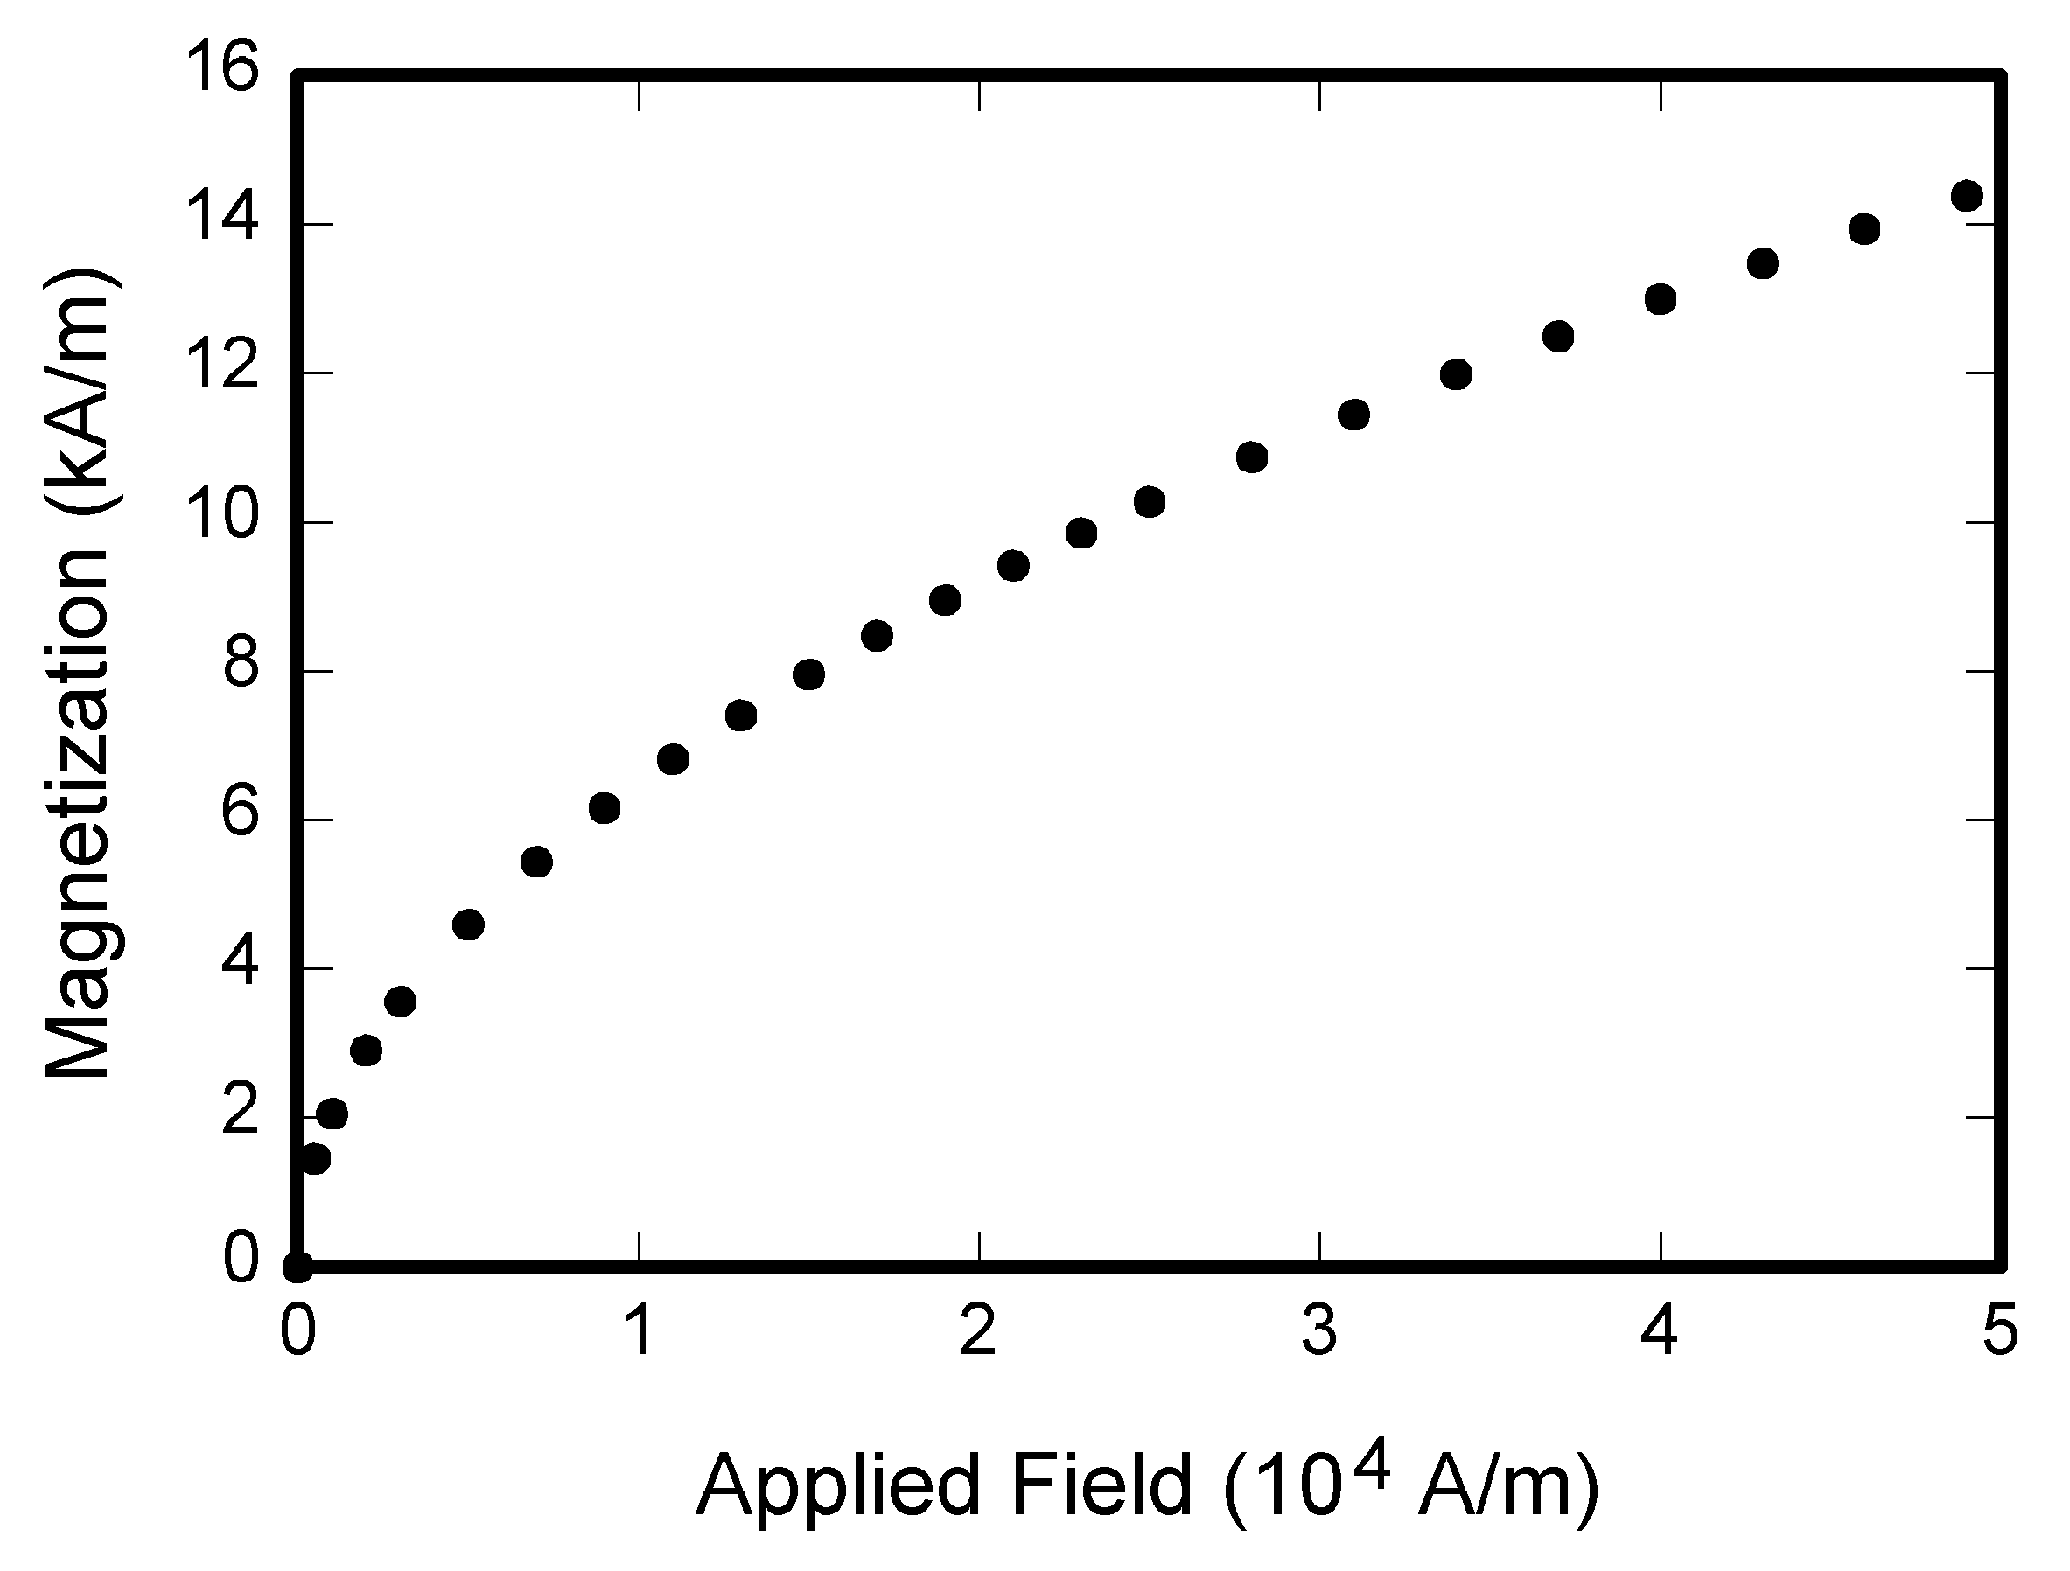
\includegraphics[width=.9\linewidth]{figures/fig1.png}
    \caption{示例图片}
  \end{figure}
\end{columns}
\end{frame}

\begin{frame}{引用与结论}
\begin{enumerate}
  \item 参考文献会以中南蓝显示，例如 \citep{langley00}。
  \item 通过 `\textcolor{csu}{\bfseries}` 可强调关键结论。
  \item 直接使用 XeLaTeX 编译即可获得中文、数学和校徽背景支持。
\end{enumerate}
\end{frame}

\begin{frame}{参考文献}
  \renewcommand*{\bibfont}{\footnotesize}
  \bibliography{ref}
  \bibliographystyle{apalike}
\end{frame}

\begin{frame}
  \begin{center}
    {\Huge\calligra Thanks!}
  \end{center}
\end{frame}

\end{document}
